\documentclass{beamer} [10.12.2024]
\usepackage[utf8]{inputenc}
\usepackage[ngerman]{babel}
\usepackage[T1]{fontenc}
\usepackage{lmodern}
\usepackage{array}
\usepackage{graphicx}
\usepackage{mathtools}
\usepackage{amsmath} 
\usepackage{subfig}
\usepackage{hyperref}

\captionsetup[figure]{labelformat=simple, labelsep=colon}
\renewcommand\thefigure{\arabic{figure}}
\setbeamertemplate{caption}[numbered]
\bibliographystyle{plain} 

\definecolor{lightblue}{rgb}{0.47, 0.47, 0.85}


\mode<presentation>{%
	\usetheme{Berlin}
	\setbeamercovered{transparent}
}


\title{CZGame}
\subtitle{Ein interaktives Point-and-Click Spiel}
\author{Jeje C., Gustav G., Rita G., Jonas G., Jonas L., Sophie P., Emil R., Antonia V., Arthur W., Ashley W.}
\institute[CZG]{Carl-Zeiss-Gymnasium Jena}
\date{\today}

\begin{document}
	
	\begin{frame}
		\titlepage
	\end{frame}
	
	\begin{frame}{Gliederung}
		\tableofcontents[pausesections]
	\end{frame}
	
	\section{Spielidee}
	\begin{frame}
	\begin{center}
		\Huge Einleitung
	\end{center}
\end{frame}

\begin{frame}
	\frametitle{Euer Titel}
\end{frame}

\begin{frame}{Aufbau des Spiels}
	\begin{figure}
		\centering
		\includegraphics[width=.9\textwidth]{figures/start.png}
		\caption[Startscreen]{Startszene unseres Spiels \glqq CZGame\grqq}
		\label{fig:Startscreen}
	\end{figure}
\end{frame}

\begin{frame}{Aufbau des Spiels}
	\begin{figure}
		\centering
		\includegraphics[width=.9\textwidth]{figures/f1}
		\caption[Vorgeschichte]{Vorgeschichte des Spiels}
		\label{fig:Vorgeschichte}
	\end{figure}
\end{frame}

\begin{frame}{Aufbau des Spiels}
	\begin{figure}
		\centering
		\includegraphics[width=.9\textwidth]{figures/f2}
		\caption[Fachschaften]{Auswahl seiner Fachschaft}
		\label{fig:Fachschaftauswahl}
	\end{figure}
\end{frame}

\begin{frame}{Aufbau des Spiels}
	\begin{figure}
		\centering
		\includegraphics[width=.9\textwidth]{figures/anleitung}
		\caption[Tutorial]{Tutorial des Spiels}
		\label{fig:Tutorial}
	\end{figure}
\end{frame}

\begin{frame}{Aufbau des Spiels}
	\begin{figure}
		\centering
		\includegraphics[width=.9\textwidth]{figures/f4}
		\caption[Foyer]{Start des \glqq CZGame\grqq \ im Foyer}
		\label{fig:Foyer}
	\end{figure}
\end{frame}

\begin{frame}{Aufbau des Spiels}
	\begin{figure}
		\centering
		\includegraphics[width=.9\textwidth]{figures/Chemiegang}
		\caption[Chemiegang]{Beispiel eines Ganges (hier der Chemiegang)}
		\label{fig:Chemiegang}
	\end{figure}
\end{frame}

\begin{frame}{Aufbau des Spiels}
	\begin{figure}
		\centering
		\includegraphics[width=.9\textwidth]{figures/inforaum}
		\caption[Informatikraum]{Beispiel eines Raumes (hier der Informatikraum)}
		\label{fig:Informatikraum}
	\end{figure}
\end{frame}

\begin{frame}{Aufbau des Spiels}
	\begin{figure}
		\centering
		\includegraphics[width=.9\textwidth]{figures/inventar}
		\caption[Inventar]{Geöffnetes Inventar mit Items}
		\label{fig:Inventar}
	\end{figure}
\end{frame}

\begin{frame}{Aufbau des Spiels}
	\begin{figure}
		\centering
		\includegraphics[width=.9\textwidth]{figures/kleinestreppenhaus}
		\caption[kleines Treppenhaus]{Beispiel eines kleines Treppenhauses}
		\label{fig:kleines Treppenhaus}
	\end{figure}
\end{frame}
	
	\section{Grafikdesign}
	\begin{frame}
	\begin{center}
		\Huge Grafikdesign
	\end{center}
\end{frame}

\begin{frame}{Grafikdesign}
    \begin{figure}
        \includegraphics[width = 10cm]{bilder/Foyer_Zeittafel.png}
        \caption{Erstellung des Foyer}
    \end{figure}
\end{frame}

\begin{frame}{Grafikdesign}
    \begin{figure}
        \includegraphics[width = 10cm]{bilder/Hausmeisterraum_Zeittafel.png}
        \caption{Erstellung des Hausmeisterraumes}
    \end{figure}
\end{frame}

\begin{frame}{Grafikdesign}
    \begin{figure}
        \includegraphics[width = 10cm]{bilder/Hausmeisterraum_Details.png}
        \caption{Details im Hausmeisterraum}
    \end{figure}
\end{frame}




\begin{frame}{Grafikdesign}
	\begin{minipage}[v]{0.32 \textwidth}
		\begin{figure}
			\includegraphics[width=\textwidth]{bilder/Bioraum.png}
			\caption[Bioraum]{\newline Der Bioraum}
			\label{fig:Bioraum}
		\end{figure}
	\end{minipage}
\hfill
\begin{minipage}[v]{0.32 \textwidth}
	\begin{figure}
		\includegraphics[width=\textwidth]{bilder/Info-Raum.png}
		\caption[Inforaum]{\newline Der Inforaum}
		\label{fig:Inforaum}
	\end{figure}
\end{minipage}
\hfill
\begin{minipage}[v]{0.32 \textwidth}
	\begin{figure}
		\includegraphics[width=\textwidth]{bilder/Physikraum.png}
		\caption[Physikraum]{\newline Der Physikraum}
		\label{fig:Physikraum}
	\end{figure}
\end{minipage}

\end{frame}

\begin{frame}
    \begin{figure}
    	\begin{minipage}{0.32\textwidth}
    		\begin{figure}
    			\includegraphics[width=\textwidth]{bilder/kt_farbverlauf}
    			\label{fig:kt_farbverlauf}
    		\end{figure}
    	\end{minipage}
        \hfill
        \begin{minipage}[v]{0.32\textwidth}
            \begin{figure}
                \includegraphics[width=\textwidth]{bilder/kt_schule.png}
                \label{fig:kt_schule}
            \end{figure}
        \end{minipage}
        \hfill
        \begin{minipage}[v]{0.3\textwidth}
            \begin{figure}
                \includegraphics[width=\textwidth]{bilder/kt_tetris.png}
                \label{fig:kt_tetris}
            \end{figure}
        \end{minipage}
        \caption{drei unterschiedliche kleine Treppenhäuser}
    \end{figure}
\end{frame}

\begin{frame}
	\frametitle{Gang- und Raumszenen}
	\begin{itemize}
		\item für jede Szene gibt es eine eigene Klasse
		\item Szenenwechsel per Pfeil in den Gängen
		\item Eintritt in Räume über die Türen
		\item in jeder Szene taucht der Spieler auf
	\end{itemize}
\end{frame}

\begin{frame}
	\begin{figure}
		\includegraphics[width = 11 cm]{bilder/Chemiegang.png}
		\caption{Chemiegang}
	\end{figure}
\end{frame}

\begin{frame}
	\frametitle{Aufbau der Szenenklassen}
	\begin{figure}
		\includegraphics[width = 11 cm]{bilder/CodeSzene.png}
		\caption{Beispielcode (Chemiegang)}
	\end{figure}
\end{frame}

\begin{frame}
	\frametitle{Das Pfeilobjekt}
	\begin{minipage}{0.45\textwidth}
		\begin{itemize}
			\item formale Parameter:
			\begin{itemize}
				\item Originalszene
				\item Zielszene
				\item Richtung
			\end{itemize}
			\item getSprite(int Richtung)
			\item Festlegen der Position des Pfeils abhängig von der angegebenen Richtung
		\end{itemize}
	\end{minipage}
	\begin{minipage}{0.45\textwidth}
		\begin{figure}
			\includegraphics[width = 5 cm]{bilder/Pfeile.png}
			\caption{Pfeile}
		\end{figure}
	\end{minipage}
\end{frame}

\begin{frame}
	\frametitle{Das Pfeilobjekt}
	\textbf{Updatefunktion}
	\begin{itemize}
		\item Wenn das Objekt angeklickt wird:
		\begin{itemize}
			\item Austausch der alten gegen die neue Szene im Szenenstapel
			\item Timer für das Inventar
		\end{itemize}
	\end{itemize}
\end{frame}

\begin{frame}
	\frametitle{Das Türobjekt}
	\begin{minipage}{0.65\textwidth}
		\begin{itemize}
			\item formale Parameter:
			\begin{itemize}
				\item x-Koordinate
				\item y-Koordinate
				\item Originalszene
				\item Zielszene
			\end{itemize}
			\item unsichtbares Objekt
			\item Updatefunktion
			\begin{itemize}
				\item Austausch der Szenen im Szenenstapel
			\end{itemize}
		\end{itemize}
	\end{minipage}
	\begin{minipage}{0.3\textwidth}
		\begin{figure}
			
\includegraphics[width = 3.5 cm]{bilder/Tür.png}
			\caption{Tür}
		\end{figure}
	\end{minipage}
\end{frame}

\begin{frame}
	\frametitle{Position des Spielers}
	\begin{minipage}{0.6\textwidth}
		\begin{itemize}
			\item Methode getRandomX()
			\begin{itemize}
				\item Festlegen einer zufälligen x-Koordinate für die Spielfigur
			\end{itemize}
		\end{itemize}
	\end{minipage}
	\begin{minipage}{0.35\textwidth}
		\begin{figure}
			
\includegraphics[width = 3.75 cm]{bilder/Spieler.png}
			\caption{Spielfigur}
		\end{figure}
	\end{minipage}
\end{frame}

\begin{frame}
	\begin{figure}
		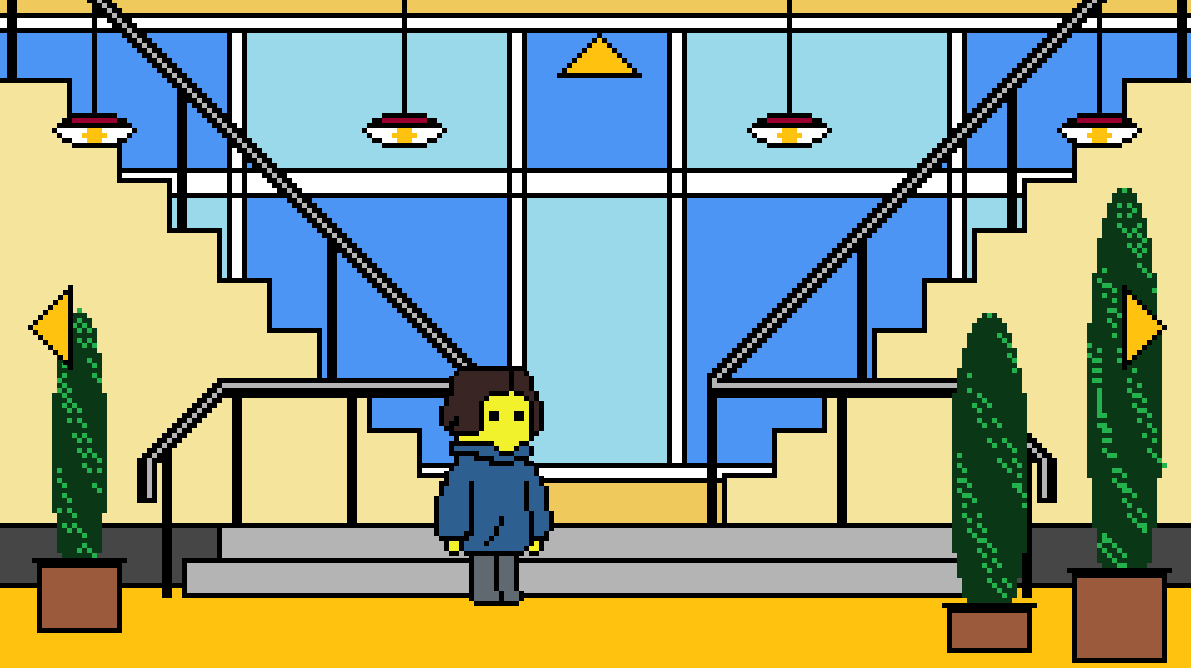
\includegraphics[width = 11 cm]{bilder/Foyer.png}
		\caption{Foyer}
	\end{figure}
\end{frame}

	
	\section{Item und Charakterdesign}
	\begin{frame}
	\begin{center}
		\Huge Item und Charakterdesign
	\end{center}
\end{frame}

\begin{frame}
	\frametitle{Euer Titel}
\end{frame}

\begin{frame}
	\frametitle{Euer Titel}
\end{frame}

\begin{frame}
	\frametitle{Euer Titel}
\end{frame}

\begin{frame}
	\frametitle{Euer Titel}
\end{frame}
	
	\section{Minigames}
	\begin{frame}
	\begin{center}
		\Huge Minigames
	\end{center}
\end{frame}

\begin{frame}
	\frametitle{Euer Titel}
\end{frame}

\begin{frame}
	\frametitle{Euer Titel}
\end{frame}

\begin{frame}
	\frametitle{Euer Titel}
\end{frame}

\begin{frame}
	\frametitle{Euer Titel}
\end{frame}

\begin{frame}
	\frametitle{Euer Titel}
\end{frame}

\begin{frame}
	\frametitle{Euer Titel}
\end{frame}

\begin{frame}
	\frametitle{Euer Titel}
\end{frame}
	
	\section{Kampf}
	\begin{frame}
	\begin{center}
		\Huge Kampf
	\end{center}
\end{frame}

\begin{frame}
	\frametitle{Das Kampfkonzept}
		\begin{itemize}
		\item Klick auf den Lehrer $\rightarrow$ Kampf startet
		\item Schüler und Lehrer im Kampfhintergrund 
		\item Schüler-Angriff
		\item Lehrer verteidigt oder nicht
		\item Lehrer-Angriff
		\item Schüler verteidigt innerhalb von 4s ich änder eh nochmal
	\end{itemize}
\end{frame}

\begin{frame}
	\frametitle{Lösungsansätze}
	Erster Lösungsansatz: while-Schleife
	Hier kommt eine Aufzählung hin.
\end{frame}

\begin{frame}
	\frametitle{Funktion: getItems}
	\begin{figure}
		\centering
		\includegraphics[width=.8\textwidth]{bilder/GetItems.png}
		\caption{Ausschnitt der Funktion getItems (Bildschirmfoto des Projektes)}
		\label{fig:agi}
	\end{figure}
\end{frame}

\begin{frame}
	\frametitle{Lehrer-Funktion}
		\begin{figure}
		\centering
		\includegraphics[width=.6\textwidth]{bilder/Lehrer-Funktion.png}
		\caption{Ausschnitt der Funktion getItems (Bildschirmfoto des Projektes)}
		\label{fig:alf}
	\end{figure}
\end{frame}

\begin{frame}
	\frametitle{Angriff und Verteidigung}
	Das kommt dann noch.
\end{frame}

\begin{frame}
	Erst erklären warum Idee I nicht funktioniert.\\
	Dann Idee zwei erklären.\\
	\begin{itemize}
		\item Update Funktion noch einmal einführen
		\item warum sie uns hilft
		\item verschiedene updates erklären
		\item noch draw Funktion ansprechen
	\end{itemize}
\end{frame}

\begin{frame}
	\frametitle{Methode 2}
	\begin{figure}
		\centering
		\includegraphics[width=.9\textwidth]{bilder/InfoKampfMethode2.png}
		\caption{Warum Methode 1 nicht funktioniert}
		\label{fig:erklaerungMethode2}
	\end{figure}
\end{frame}

\begin{frame}
	\frametitle{Die update() Funktion}
	\begin{figure}
		\centering
		\includegraphics[width=.9\textwidth]{bilder/InfoUpdates.png}
		\caption{Wie update() funktioniert}
		\label{fig:erklaerungUpdates}
	\end{figure}
\end{frame}

\begin{frame}
	\begin{algorithm}[H]
		\begin{algorithmic}[1]
			\STATE Hintergrundbild
			\STATE Variablen festsetzen
			\STATE Lehrer $\gets$ new LehrerObject(FACHSCHAFT)
			\STATE button zum Kampfabbruch
			\STATE music $\gets$ Kampfmusik
		\end{algorithmic}
		\caption{KampfScene(FACHSCHAFT) pseudocode}
		\label{alg:SceneKonstruction}
	\end{algorithm}
\end{frame}

\begin{frame}
	\begin{algorithm}[H]
		\begin{algorithmic}[1]
			\IF {LehrerLeben $\leq$ 0}
				\STATE Gewonnen
				\STATE Dekrementiere UebrigeLehrer
				\STATE Beende Kampf
			\ENDIF
			\IF {PlayerLeben $\leq$ 0 $\vee$ |PlayerItems| = 0}
				\STATE Verloren
				\STATE Beende Kampf
			\ENDIF
		\end{algorithmic}
		\caption{KampfScene.update() pseudocode}
		\label{alg:SceneUpdate}
	\end{algorithm}
\end{frame}

\begin{frame}
	\begin{algorithm}[H]
		\begin{algorithmic}[1]
			\IF {timer $\neq$ 0}
			\STATE draw timer 
			\ENDIF
		\end{algorithmic}
		\caption{KampfScene.draw() pseudocode}
		\label{alg:SceneDraw}
	\end{algorithm}
\end{frame}

\begin{frame}
	\begin{algorithm}[H]
		\begin{algorithmic}[1]
			\IF {Turn = LehrerAngriff}
				\STATE ZwischenSchaden $\gets$ LehrerAngriff()
				\IF {ItemBenutzt} 
					\STATE DisplayItem()
				\ENDIF
				\STATE timer $\gets$ 4 Sekunden
				\STATE Turn $\gets$ PlayerVerteidigung
			\ELSIF {Turn = LehrerVerteidigung}
				\STATE LehrerLeben -= LehrerVerteidigung(Zwischenschaden)
				\STATE Turn $\gets$ PlayerAngriff
			\ENDIF
		\end{algorithmic}
		\caption{LehrerObject.update() pseudocode}
		\label{alg:LehrerUpdate}
	\end{algorithm}
\end{frame}

\begin{frame}
	\begin{algorithm}[H]
		\begin{algorithmic}[1]
			\IF {imKampf}
			\IF {Turn = PlayerAngriff}
			\STATE ZwischenSchaden $\gets$ PlayerAngriff(clickedItem)
			\STATE Turn $\gets$ LehrerVerteidigung
			\ELSIF {Turn = PlayerVerteidigung}
			\STATE PlayerLeben -= PlayerVerteidigung(Zwischenschaden, clickedItem)
			\STATE Turn $\gets$ LehrerAngriff
			\ENDIF
			\ENDIF
		\end{algorithmic}
		\caption{PlayerObject.update() pseudocode}
		\label{alg:PlayerUpdate}
	\end{algorithm}
\end{frame}

\begin{frame}
	\begin{algorithm}[H]
		\begin{algorithmic}[1]
			\IF {turn = Angriff}
			\STATE draw \dq Angriff"
			\ELSIF {turn = Verteidigung}
			\STATE draw "Verteidigung"
			\ENDIF
			\STATE draw Leben
		\end{algorithmic}
		\caption{draw() pseudocode}
		\label{alg:Draw}
	\end{algorithm}
\end{frame}


	\section{Spielende}
	\begin{frame}
	\begin{center}
		\Huge Spielende
	\end{center}
\end{frame}

\begin{frame}
	\frametitle{Spielende}
	\centering
    		\begin{figure}
    			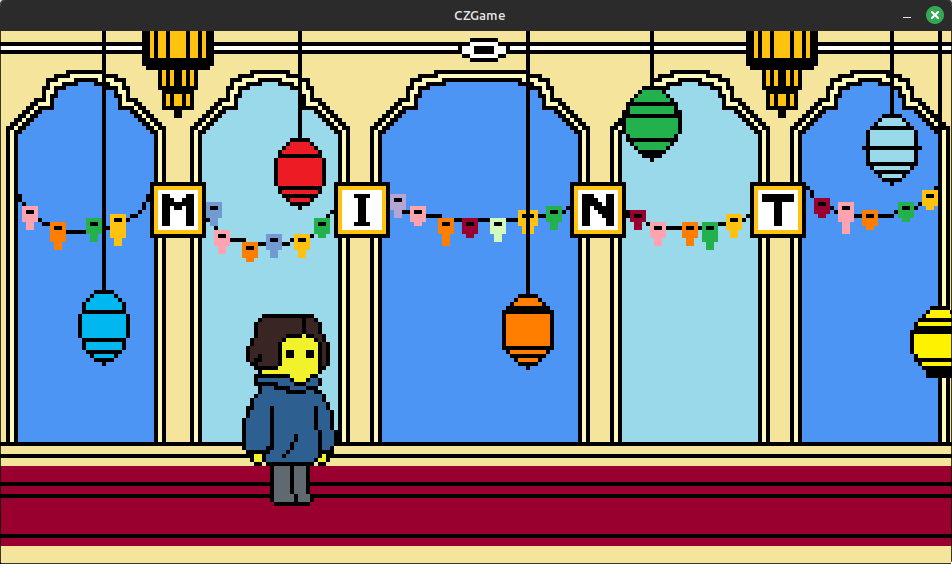
\includegraphics[width=\textwidth]{../präsi/bilder/EndScene.png}
    			\caption{EndScene}
    		\end{figure}
\end{frame}


	\section{Sound}
	\begin{frame}
	\begin{center}
		\Huge Sound
	\end{center}
\end{frame}



	
\section*{}
	
	\begin{frame}
		\begin{center}
			\Large\textbf{Vielen Dank für Ihre Aufmerksamkeit!}
		\end{center}
		
		\vspace{0,5cm}
		
		\begin{block}{Fragen}
			Wir stehen Ihnen jetzt gerne für Fragen zur Verfügung.
		\end{block}
		
		\vspace{1cm}
		
		\begin{flushright}
			\footnotesize{Diese Präsentation wurde mit \LaTeX{} erstellt.}
		\end{flushright}
	\end{frame}
	
	
	\section*{}
	\begin{frame}[allowframebreaks]{Literaturverzeichnis} 
		%% \nocite{*}
		%% \bibliography{verzeichnis} 
	\end{frame}
	
	\section*{}
	\begin{frame}[allowframebreaks]{Abbildungsverzeichnis} 
		\begin{itemize}
			\item[Abb. 1] 
			\item[Abb. 2] 
			\item[Abb. 3] 
			\item[Abb. 4] 
			\item[Abb. 5] 
		\end{itemize}
	\end{frame}
	
\end{document}